\section{Fire !(50pts)}
Naviya在练习她的玫瑰礼花炮弹,她首先测试一下低功率火力的情况,她选择了一块平地作为测试场地。已知重力加速度为\(g\),炮弹的初速度为\(v\)。
\begin{enumerate}
	\item 如图\ref{fire1} 所示,Naviya发现她的炮弹的轨迹是抛物线,并且无意中发现似乎发射点到抛物线的焦点的距离一直是一个定值,并且还发现抛物线的准线一直没有发生改变,请你帮她证明这现象的正确性。(10pts)
	\begin{figure}[htbp]
	\centering
	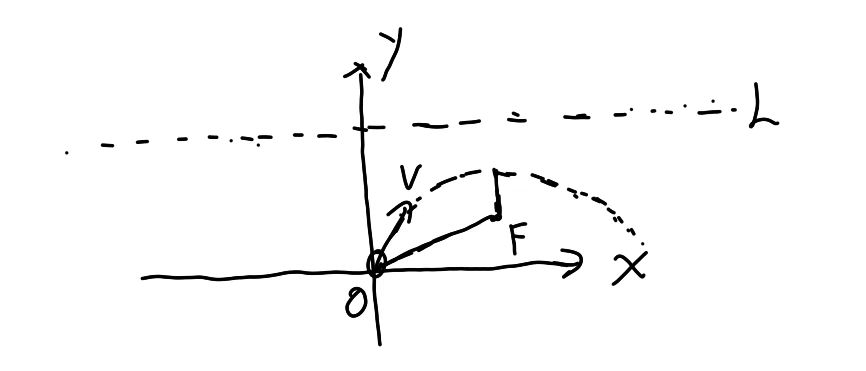
\includegraphics[width=0.5\textwidth]{fire1}
	\caption{炮弹轨迹示意图.}
	\label{fire1}
	\end{figure}
	\item 接着她想测试一下她的范围在限定的速度下能达到的最远的范围,也就是需要求出所有的抛物线的包络线,她猜测包络线也是一个抛物线,也就是对于任意轨迹上的任意一点P,到某一个点的距离始终小于或等于(可以取到等号)到某一条直线的距离。请你帮她找到这个点和这个直线,并且证明她的猜测是正确的,在写出包络线方程。(推荐几何方法解题哦,不过你也可以直接数学解析爆算但可能对下面题没有启发性)(10pts)
	\item 接着她开始加大炮塔的功率,使得炮弹的速度可以飞向太空中,但并没有超过第二宇宙速度。如图\ref{fire2}所示,她发现此时炮弹的轨迹变成了椭圆,她想知道现在发射点到焦点的距离是否还是一个定值?论证你的结论并帮她求出此时能达到的所有范围的包络线方程。(已知万有引力常数为\(G\),地球质量为\(M\),地球半径为\(R\),坐标原点设在地球中心,此问你可以不用考虑地球的碰撞体积)(20pts)
	\item 定义Naviya炮弹最小速度为使得第三问中的包络线恰好与地球表面相切的速度大小,求出这个速度的表达式。(10pts)
	\item 思考题:如果Naviya炮弹的速度超过了第二宇宙速度,那么包络线又会是什么?(0pts)
	\begin{figure}[htbp]
	\centering
	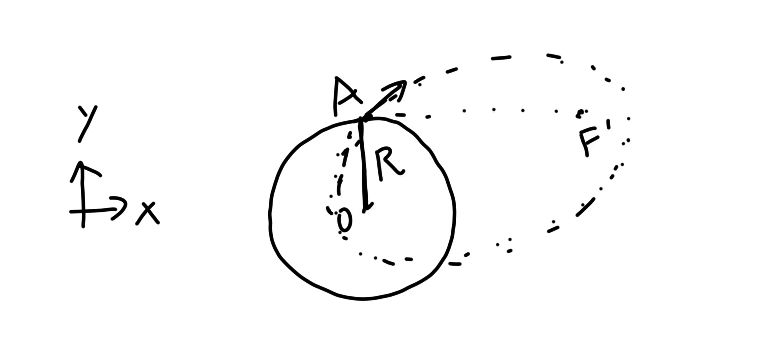
\includegraphics[width=0.5\textwidth]{fire2}
	\caption{炮弹轨迹示意图.}
	\label{fire2}
	\end{figure}
\end{enumerate}